\documentclass[a4j]{ujarticle}
\renewcommand{\baselinestretch}{0.85}
\usepackage[top=1.5cm, bottom=1.5cm, left=1.5cm, right=1.5cm]{geometry}
\usepackage{xcolor}
\usepackage[dvipdfmx]{graphicx, hyperref}
\usepackage{listings}
\usepackage{multirow}
\usepackage{siunitx}
\usepackage{subfig}
\usepackage{url}
\usepackage{listings}
\usepackage{caption,stackengine}

\colorlet{punct}{red!60!black}
\definecolor{background}{HTML}{EEEEEE}
\definecolor{delim}{RGB}{20,105,176}
\colorlet{numb}{magenta!60!black}

\newcommand{\Sref}[1]{\mbox{\ref{sec:#1}}}
\newcommand{\Tref}[1]{\mbox{表\ref{tab:#1}}}
\newcommand{\Eref}[1]{\mbox{式(\ref{eq:#1})}}
\newcommand{\Fref}[1]{\mbox{図\ref{fig:#1}}}
\renewcommand{\lstlistingname}{ソースコード}
\newcommand{\Lref}[1]{\mbox{ソースコード\ref{lst:#1}}}
\newcommand{\bhline}[1]{\noalign{\hrule height #1}}

\hypersetup{
	setpagesize=false,
	bookmarksnumbered=true,
	bookmarksopen=true,
	colorlinks=true,
	linkcolor=black,
	citecolor=black
}

\begin{document}
    \begin{flushright}
        MDLab GM資料\\
        22年5月31日(火)
    \end{flushright}

    \begin{center}
        {\Large	腹部超音波画像からの腫瘍検出}
    \end{center}

    \begin{flushright}
        {\large B4 原 英吾}\\
    \end{flushright}

    \section{研究背景および目的}
    \begin{figure}[h]
        \begin{minipage}{.59\textwidth}
            \begin{itemize}
                \item 背景
                \begin{itemize}
                    \item 器具の操作と診断を同時に行わなければならず高難易度
                    \item 肝臓は沈黙の臓器と呼ばれ初期には自覚症状がほとんどない
                    \begin{itemize}
                        \item 症状を自覚している時には重症化している場合が多い
                    \end{itemize}
                    \item 機械学習による診断のサポート
                    \begin{itemize}
                        \item 良性・悪性を見分けることが重要視される
                        \item \Fref{ex}の様に明らかなラベル不足\footnotemark[1]のある画像が存在する
                    \end{itemize}
                \end{itemize}
                \item 目的
                \begin{itemize}
                    \item 既存の研究を踏まえたモデルの精度向上
                    \begin{itemize}
                        \item 良性・悪性判別の高精度化
                    \end{itemize}
                    \item 超音波支援システムの開発
                    \begin{itemize}
                        \item 早期発見につながると良い
                    \end{itemize}
                \end{itemize}
            \end{itemize}
        \end{minipage}
        \begin{minipage}{.39\textwidth}
            \centering
            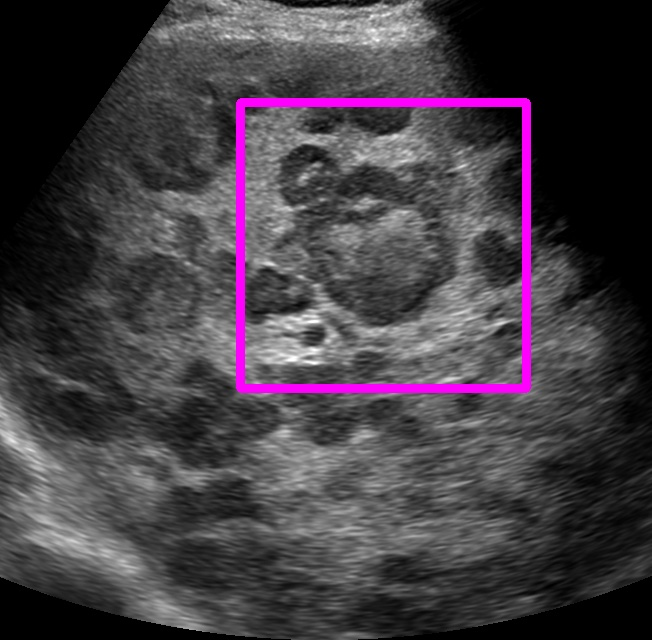
\includegraphics[width=.9\linewidth]{../fig/pseudo_a.png}
            \caption{ラベル不足のある診断画像例}
            \label{fig:ex}
        \end{minipage}
    \end{figure}

    \footnotetext[1]{今回は\Fref{ex}の様なアノテーションが不足しているものを指す}
    \addtocounter{footnote}{1}

    \section{これまでの研究のまとめ}
        \begin{itemize}
            \item データセット
            \begin{itemize}
                \item 国立研究開発法人日本医療研究開発機構(AMED)\footnote{\url{https://www.amed.go.jp/}}が提供している延べ8万枚に及ぶ以下のデータが付随
                \begin{itemize}
                    \item 腹部超音波画像,ROI
                    \item 年齢,性別
                \end{itemize}
                \begin{figure}[h]
                    \centering
                    \subfloat[性別毎の画像枚数]{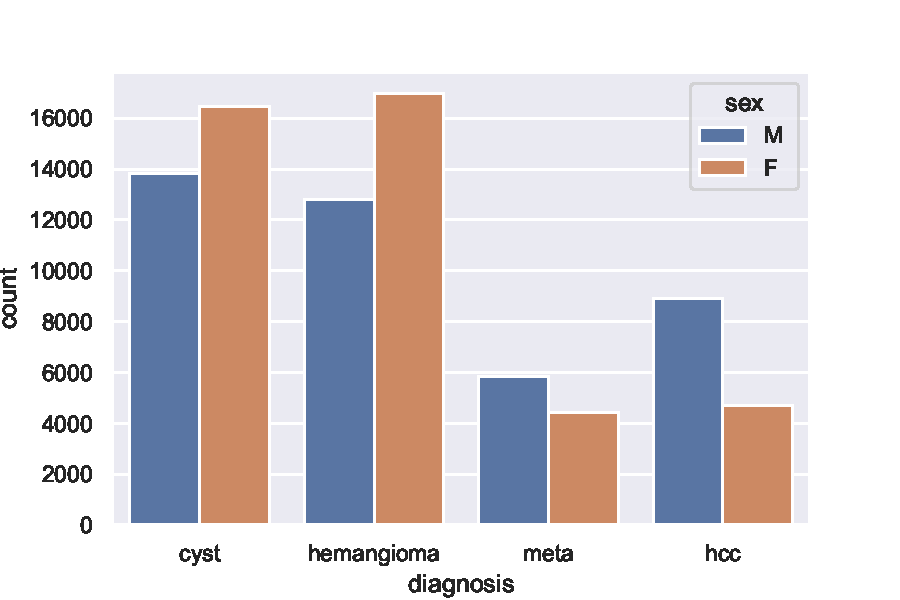
\includegraphics[width=.24\linewidth]{../fig/sex_a.pdf} \label{fig:sex}}
                    \subfloat[診断名毎の年齢分布]{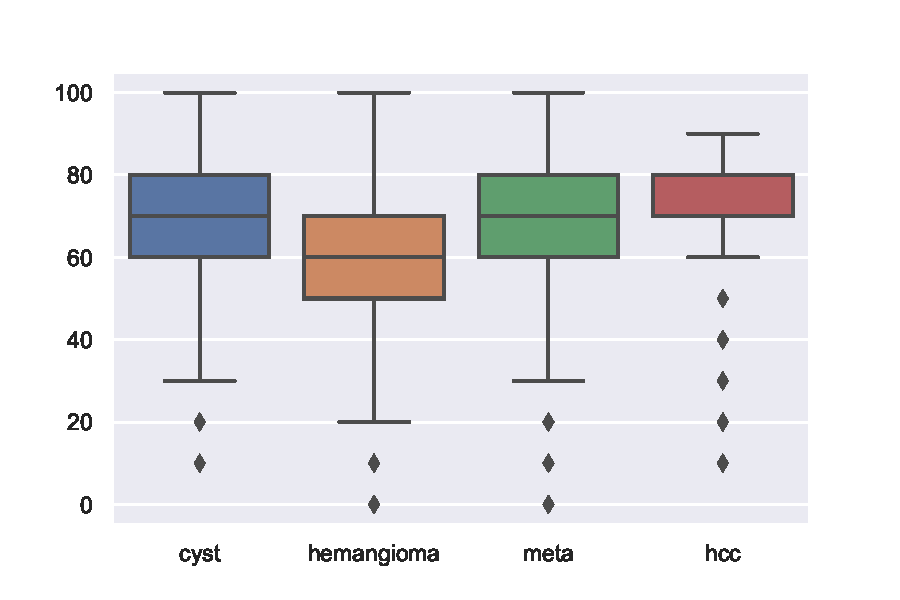
\includegraphics[width=.24\linewidth]{../fig/age_a.pdf} \label{fig:age}}
                    \subfloat[診断名毎の画像サイズの分布]{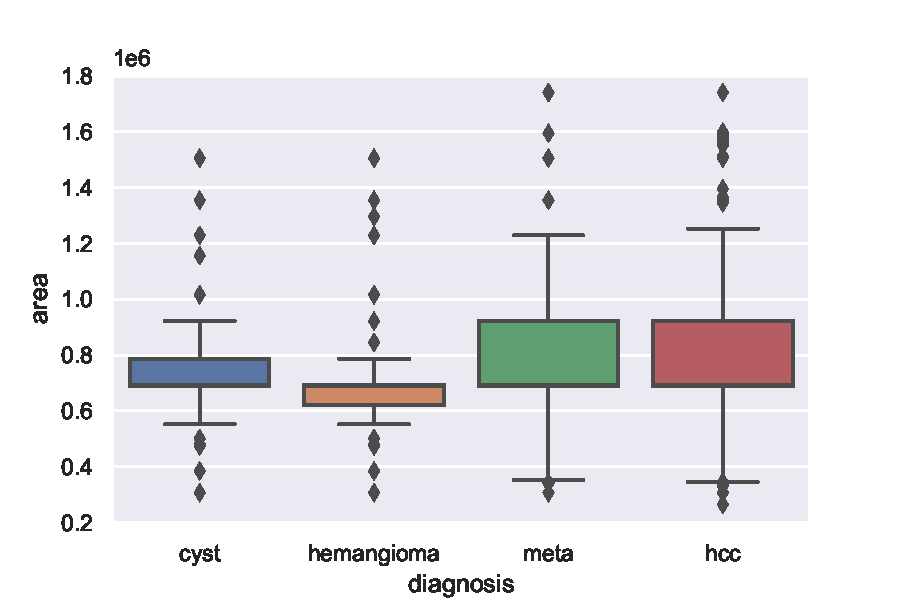
\includegraphics[width=.24\linewidth]{../fig/area_a.pdf} \label{fig:area}}
                    \subfloat[診断名毎のbboxの割合]{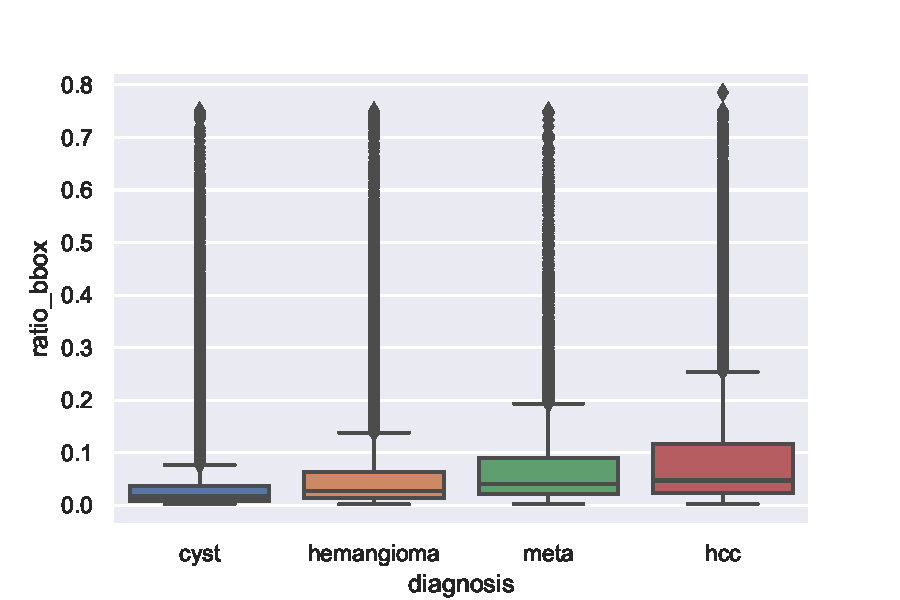
\includegraphics[width=.24\linewidth]{../fig/ratio_bbox_a.pdf} \label{fig:ratio}}
                    \caption{データセットにおけるデータの分布}
                \end{figure}
                \item 性別(\Fref{sex})
                \begin{itemize}
                    \item HCC(肝細胞癌)は男性が罹患しやすい
                    \begin{itemize}
                        \item 昔は男性の方が飲酒・タバコが多く癌に罹りやすかったという時代背景があるかもしれない
                    \end{itemize}
                    \item hemangioma(血管腫)は女性が罹患しやすい
                    \item Meta(転移性肝癌)は他の症状よりも少ない
                \end{itemize}
                \item 年齢(\Fref{age})
                \begin{itemize}
                    \item cyst(単純嚢胞),hemangioma(血管腫)の分布にははあまり特徴がない
                    \item hemangioma(血管腫)は比較的若年層でも罹患する
                    \item Meta(転移性肝癌)における0歳はラベルミスである可能性が高い
                    \item HCC(肝細胞癌)は比較的高齢者が罹患しやすい
                \end{itemize}
                \item 画像サイズ(\Fref{area})
                \begin{itemize}
                    \item hemangioma(血管腫)は比較的画像サイズが統一されている
                    \begin{itemize}
                        \item 腫瘍の大きさが血管に依存するためあまり偏りが生じていない?
                    \end{itemize}
                \end{itemize}
                \item bboxの画像に占める割合(\Fref{ratio})
                \begin{itemize}
                    \item cyst(単純嚢胞)は他の診断と比べてbboxの割合が低い($\frac{1}{2}$程度)である
                    \item HCC(肝細胞癌)は画像に占めるbboxの割合が高い
                \end{itemize}
            \end{itemize}
        \end{itemize}

        \begin{itemize}
            \item 症状毎の特徴を調査
            \begin{figure}[h]
                \centering
                \subfloat[cyst(単純嚢胞)]{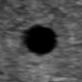
\includegraphics[width=.24\linewidth]{../fig/cyst.png} \label{fig:cyst}}
                \subfloat[hemangioma(血管腫)]{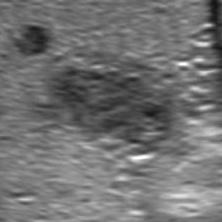
\includegraphics[width=.24\linewidth]{../fig/hemangioma.png} \label{fig:hemangioma}}
                \subfloat[Meta(転移性肝癌)]{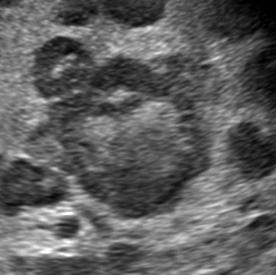
\includegraphics[width=.24\linewidth]{../fig/meta.png} \label{fig:meta}}
                \subfloat[HCC(肝細胞癌)]{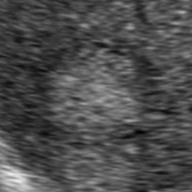
\includegraphics[width=.24\linewidth]{../fig/hcc.png} \label{fig:hcc}}
                \caption{症状毎における腫瘍の超音波画像}
            \end{figure}
            \begin{itemize}
                \item cyst(単純嚢胞) (\Fref{cyst})
                \begin{itemize}
                    \item 液体が貯留されている状態
                    \item 症状がでないことが多いため大きな腫瘍になって発見されることが多い
                    \item 嚢胞の内腔に向けて増殖するため転移することは少ない
                \end{itemize}
                \item hemangioma(血管腫) (\Fref{hemangioma})
                \begin{itemize}
                    \item 肝臓にできる良性腫瘍の中で最も多い
                    \item 女性ホルモンが原因で女性が罹患しやすいと言われているが詳しくは解明されていない
                    \item 血管が無数に絡み合うことによって出来た血管の塊であることから血流が遅いという特徴がある
                    \item 他の臓器に浸潤したり転移することは無いと言われている
                \end{itemize}
                \item Meta(転移性肝癌) (\Fref{meta})
                \begin{itemize}
                    \item 門脈を介して大腸癌などの消化器癌から転移する割合が多い
                    \item 類似したエコーパターンをもつ腫瘤が多発してみられることが多い
                \end{itemize}
                \item HCC(肝細胞癌) (\Fref{hcc})
                \begin{itemize}
                    \item 肝臓にできる悪性腫瘍の中で最も多いと言われている
                    \item 約90%がウイルス感染症が原因
                    \begin{itemize}
                        \item B型肝炎ウイルス(HBV)が約20\%
                        \item C型肝炎ウイルス(HCV)が約70\%
                    \end{itemize}
                \end{itemize}
            \end{itemize}
        \end{itemize}

        \begin{itemize}
            \item データクレンジング
            \begin{enumerate}
                \item $400 \times 400$ 以下の画像の除外
                \item Perceptual Hashを利用した類似画像の除外
                \item 青色や黄色のスケールの除去
            \end{enumerate}

            \item 提供されているデータをCOCODatasetの形式に変換
            \begin{itemize}
                \item train data : test data : val data = 67122 : 8390 : 8391
                \item 見やすいようにインデントしたファイル\footnote{\url{//aka/work/hara.e/AMED/lib/dataset/annotations/train_large.json}など}も作成
            \end{itemize}

\clearpage

            \item 1クラスと4クラス検出の学習結果
            \begin{figure}[h]
                \centering
                \subfloat[APの比較]{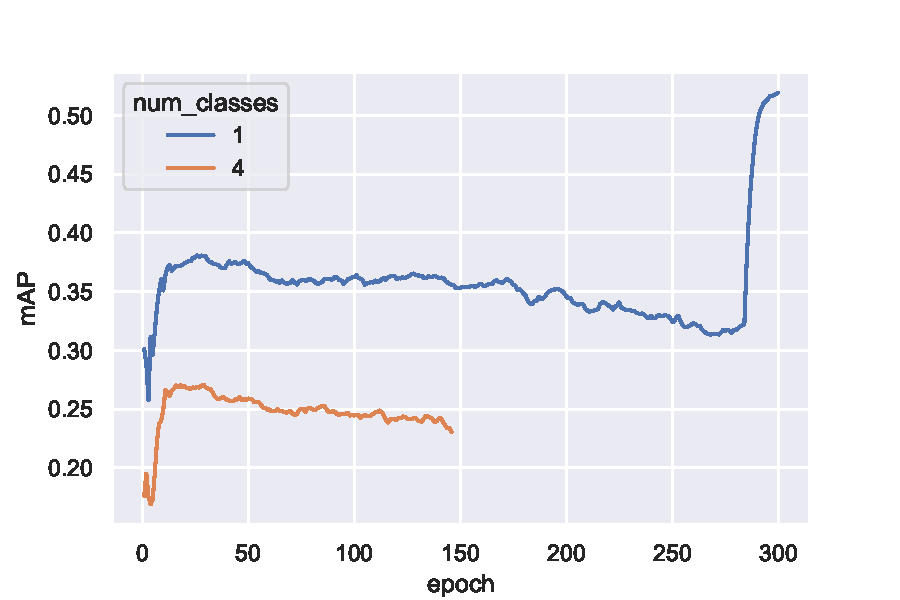
\includegraphics[width=.24\linewidth]{../fig/compare_AP.pdf} \label{fig:compare_AP}}
                \subfloat[iou\_lossの比較]{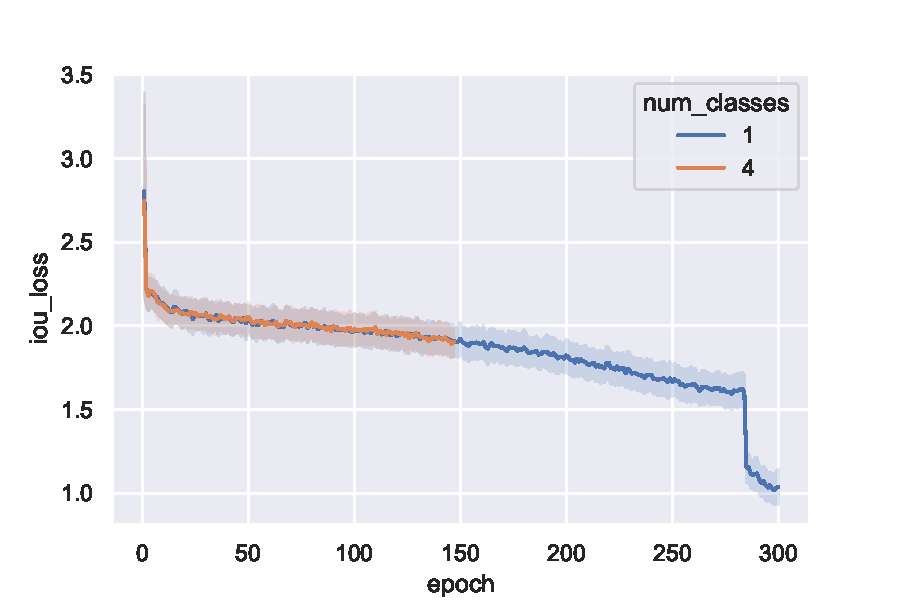
\includegraphics[width=.24\linewidth]{../fig/compare_iou_loss.pdf} \label{fig:compare_iou_loss}}
                \subfloat[cls\_lossの比較]{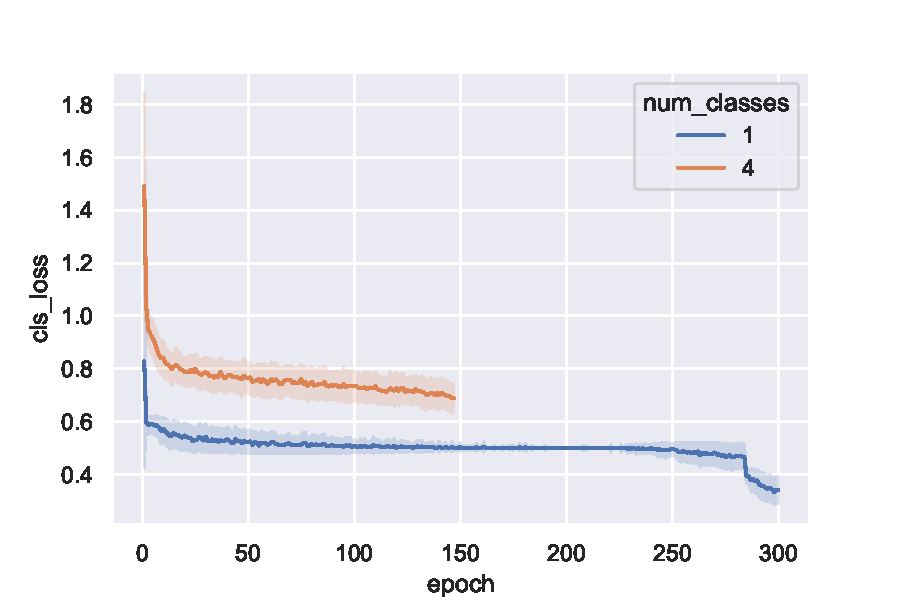
\includegraphics[width=.24\linewidth]{../fig/compare_cls_loss.pdf} \label{fig:compare_cls_loss}}
                \subfloat[4クラス分類時の混同行列]{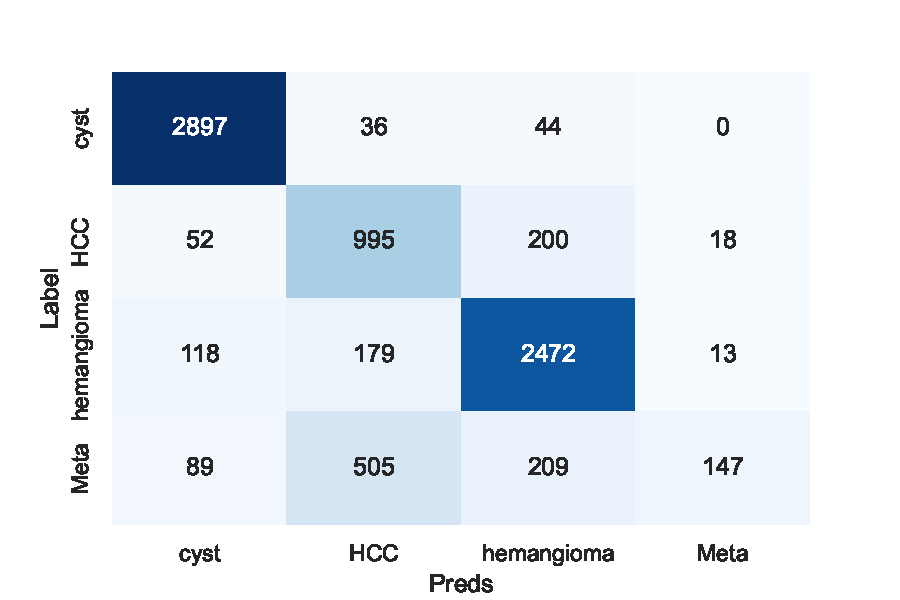
\includegraphics[width=.24\linewidth]{../fig/heatmap.pdf} \label{fig:heatmap}}
                \label{fig:compare}
                \caption{1クラス検出と4クラス検出の比較}
            \end{figure}

            \item \Fref{compare_AP}から
            \begin{itemize}
                \item 4クラス検出の方がAPが低い
            \end{itemize}
            \item \Fref{compare_iou_loss}から
            \begin{itemize}
                \item 1クラスと4クラスは,同じくらいの学習速度でiou\_lossの差異が小さい
                \item クラス数を増やしてもIoUの精度はあまり変化が無い
            \end{itemize}
            \item \Fref{compare_cls_loss}から
            \begin{itemize}
                \item 1クラスと4クラスではcls\_lossの差異が大きい
            \end{itemize}

            \begin{table}[h]
                \centering
                \caption{1クラス検出と4クラス検出の学習で得られた精度}
                \label{tab:compare}
                \begin{tabular}{cccccc|ccc|ccc}
                    & & & & & & & IoU & & & area & \\
                    model & backbone & classes & epoch & size & batch\_size & mAP & AP$_{50}$ & AP$_{75}$ & AP$_S$ & AP$_M$ & AP$_L$ \\ \hline
                    \multirow{2}{*}{YOLOX\cite{yolox}} & \multirow{2}{*}{DarkNet} & 1 & \multirow{2}{*}{300} & \multirow{2}{*}{512} & \multirow{2}{*}{64} & 0.519 & 0.839 & 0.558 & - & 0.639 & 0.631 \\
                    &  & 4 &  &  &  & 0.279 & 0.526 & 0.248 & - & 0.221 & 0.288 \\
                \end{tabular}
            \end{table}

            \item \Tref{compare}から
            \begin{itemize}
                \item APが半分程度になっている
                \item IoUが0.5の時はAPが比較的高い
                \item 4クラス検出では腫瘍が大きいものは分類しやすい傾向がある?
            \end{itemize}

            \begin{table}[h]
                \centering
                \caption{4クラス検出時の評価指標毎の値}
                \label{tab:metric}
                \begin{tabular}{c|cc|ccccc}
                    Diagnosis & 未検出数 & データ総数 & 未検出割合 & accuracy & precision & recall & f1-score \\ \hline
                    cyst & 60 & 3037 & 0.0198 & 0.8789 & 0.9179 & 0.9539 & 0.9356 \\
                    HCC & 106 & 1371 & \textcolor{red}{0.0773} & 0.4758 & \textcolor{red}{0.5801} & 0.7257 & 0.6448 \\
                    hemangioma & 180 & 2962 & \textcolor{red}{0.0608} & 0.7238 & 0.8451 & 0.8346 & 0.8398 \\
                    Meta & 71 & 1021 & \textcolor{red}{0.0695} & \textcolor{red}{0.1397} & 0.8258 & \textcolor{red}{0.1440} & \textcolor{red}{0.2452} \\ \hline
                    合計 & 417 & 8391 & 0.0497 & 0.7760 & - & 0.7760 & -
                \end{tabular}
            \end{table}

            \item \Tref{metric}から
            \begin{itemize}
                \item cyst (単純嚢胞)
                \begin{itemize}
                    \item ほぼ問題ない
                \end{itemize}
                \item hemangioma (血管腫)
                \begin{itemize}
                    \item cyst (単純嚢胞) やHCC (肝細胞癌) と誤分類してしまうことが多い
                    \item 未検出の多さが目立つ
                \end{itemize}
                \item HCC (肝細胞癌)
                \begin{itemize}
                    \item hemangioma (血管腫) と誤分類してしまうことが多い
                    \item \textcolor{red}{未検出が多い}
                \end{itemize}
                \item Meta (転移性肝癌)
                \begin{itemize}
                    \item HCC (肝細胞癌) やhemangioma (血管腫) と誤分類してしまうことが多い
                    \item \textcolor{red}{正確な予測ができていない} (予測がバラバラ) ことが多い
                \end{itemize}
            \end{itemize}

        \end{itemize}

\clearpage

    \section{前回のGMからの進捗}
        \begin{itemize}
            \item YOLOX\cite{yolox}とSimCLR\cite{simclr}からCenterNet\cite{centernet}とSimSiam\cite{simsiam}へモデルの変更
            \begin{itemize}
                \item 背景
                \begin{itemize}
                    \item YOLOX\cite{yolox}のbackboneをfinetuningして重みを固定する予定だった
                    \item 複雑なモデルのためクラスの特徴量をbackboneの外でも操作していてfinetuningするのは面倒臭い
                    \item SimCLR\cite{simclr}はバッチサイズが大きくないと効果的に学習できない
                \end{itemize}

                \begin{figure}[h]
                    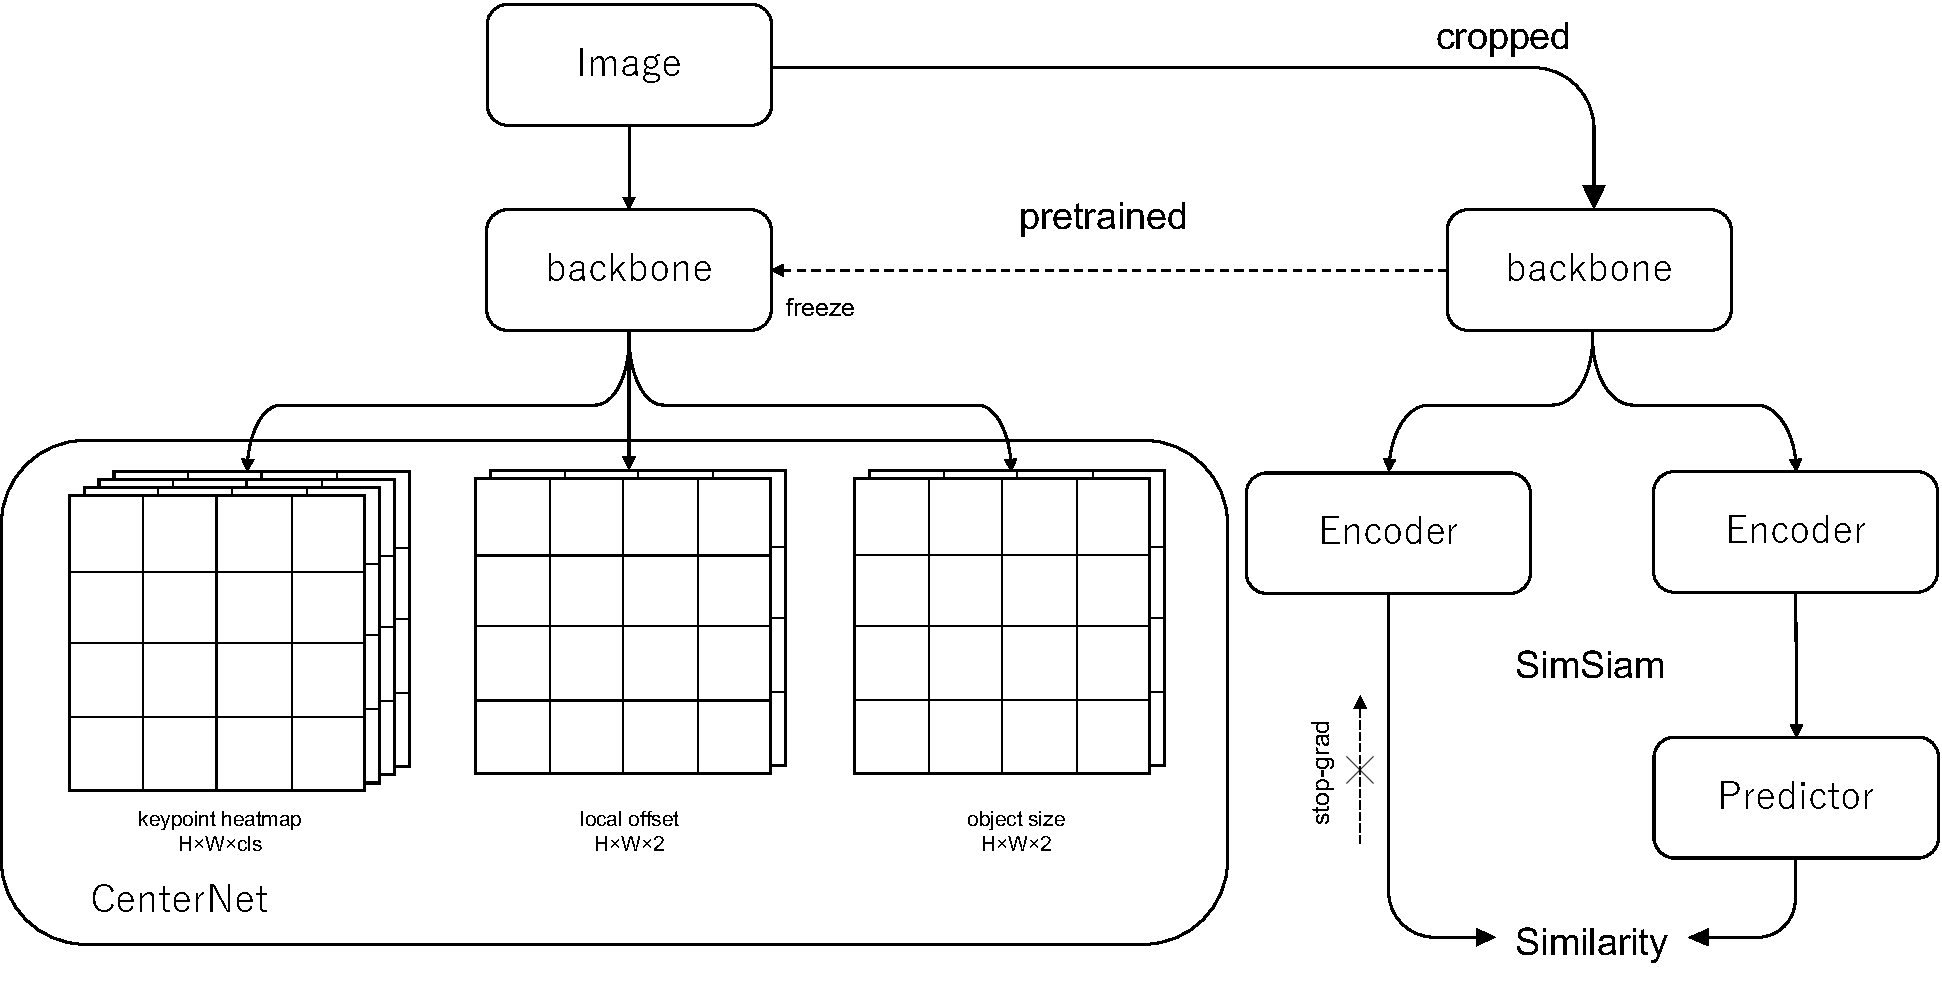
\includegraphics[width=.9\linewidth]{../fig/models.pdf}
                    \caption{CenterNet\cite{centernet}とSimSiam\cite{simsiam}の複合モデル}
                    \label{fig:models}
                \end{figure}

                \item 推論フロー
                \begin{enumerate}
                    \item SimSiam (距離学習) でbackboneをfinetuning
                    \item backboneの重みをfreeze
                    \item backboneから特徴マップを取得しCenterNet\cite{centernet}のパラメータのみを学習させる
                \end{enumerate}
            \end{itemize}
            \item SimSiamでbackbone (ResNet18) を事前学習 (途中)
            \begin{itemize}
                \item 実験で用いるSimSiam\cite{simsiam}のコード\footnote{\url{https://github.com/a5chin/AMED/blob/feature/examples/examples/simsiam.py}}を書いた
                \item 元論文のコードはbackboneのfc層しか用いられていなかった
                \item (自分の書いたコードじゃないからかもしれないが) 汚くて使いにくかった
            \end{itemize}
            \item CenterNet\cite{centernet}で4クラス検出の学習
            \begin{itemize}
                \item 実験の簡略化のため初めはMMDetectionを用いる
                \item 実験が進んでいったら自分でコードを書くつもり...

            \begin{table}[h]
                \centering
                \caption{1クラス検出と4クラス検出の学習で得られた精度}
                \label{tab:compare_models}
                \begin{tabular}{cccccc|ccc|ccc}
                    & & & & & & & IoU & & & area & \\
                    model & backbone & classes & epoch & size & batch\_size & mAP & AP$_{50}$ & AP$_{75}$ & AP$_S$ & AP$_M$ & AP$_L$ \\ \hline
                    \multirow{2}{*}{YOLOX\cite{yolox}} & \multirow{2}{*}{DarkNet} & 1 & \multirow{2}{*}{300} & \multirow{2}{*}{512} & \multirow{2}{*}{64} & 0.519 & 0.839 & 0.558 & - & 0.639 & 0.631 \\
                    &  & 4 &  &  &  & 0.279 & 0.526 & 0.248 & - & 0.221 & 0.288 \\ \hline
                    CenterNet\cite{centernet} & ResNet18 & 4 & 140 & 512 & 16 & 0.344 & 0.639 & 0.332 & - & 0.347 & 0.326
                \end{tabular}
            \end{table}

                \item 4クラスの検出ではいずれ指標でもCenterNet\cite{centernet}の方が高精度
                \begin{itemize}
                    \item Recallは同程度だがPrecisionは5\%〜10\%程高い
                    \item 中心を推定した後に高さと幅を推定する手法と円形である腫瘍の相性が良かった?
                \end{itemize}
                \item YOLOXに比べて約10倍高速
                \item LossやAP,混同行列などは間に合わなかったので後日載せる
            \end{itemize}

        \end{itemize}

\clearpage

    \section{今後の課題\&スケジュール}
        \begin{itemize}
            \item 6/14までに
            \begin{itemize}
                \item 対照学習の結果を (遅くとも6/28までに) 出すことを目標にする
                \item 結果と言ってもtestデータでPrecisionやRecallを出すところまで
                \item YOLOXの4クラス検出の結果と比較できる様にする
            \end{itemize}
        \end{itemize}

    \appendix
	\def\thesection{付録\Alph{section}}
	\section{CenterNetでの検出結果}

    \begin{figure}[h]
        \centering
        \subfloat[CenterNet]{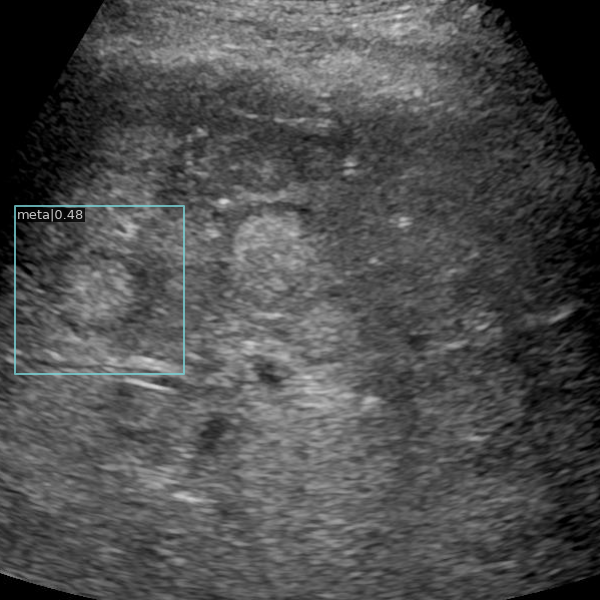
\includegraphics[width=.32\linewidth]{../fig/000020_center.png} \label{fig:meta_center}}
        \subfloat[Label]{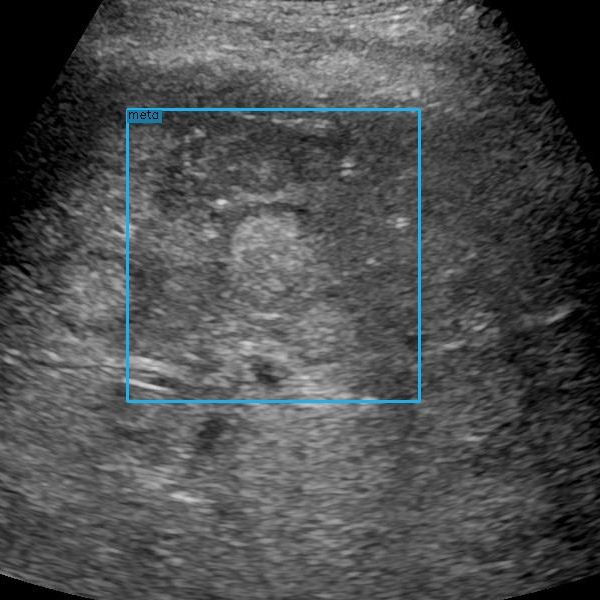
\includegraphics[width=.32\linewidth]{../fig/000020_label.png} \label{fig:meta_lael}}
        \subfloat[YOLOX]{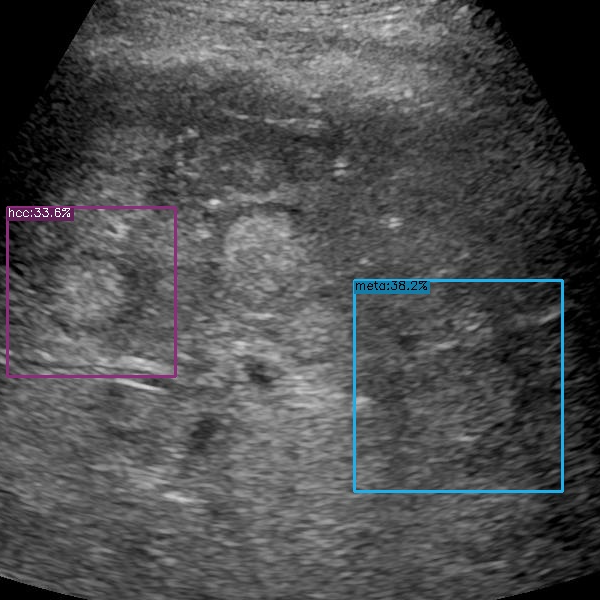
\includegraphics[width=.32\linewidth]{../fig/000020_yolox.png} \label{fig:meta_yolox}}
        \label{fig:000020}
        \caption{000020.jpgの検出結果}
    \end{figure}
    \begin{figure}[h]
        \centering
        \subfloat[CenterNet]{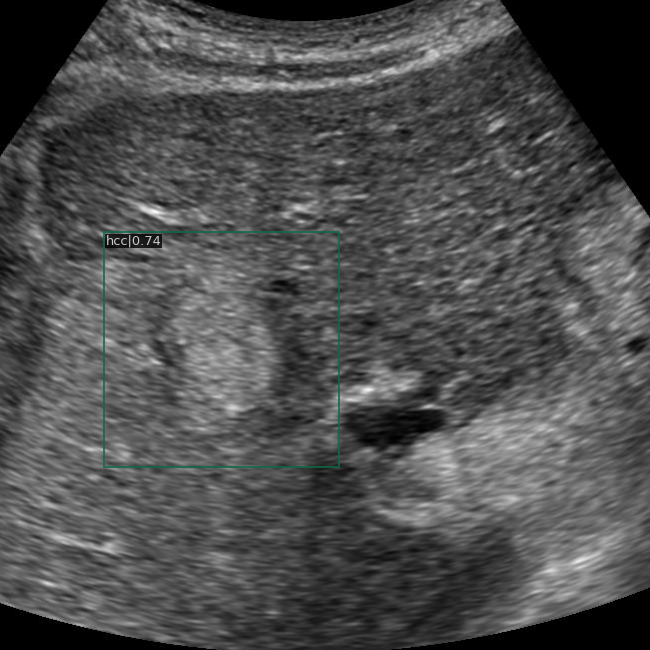
\includegraphics[width=.32\linewidth]{../fig/000814_center.png} \label{fig:hcc_center}}
        \subfloat[Label]{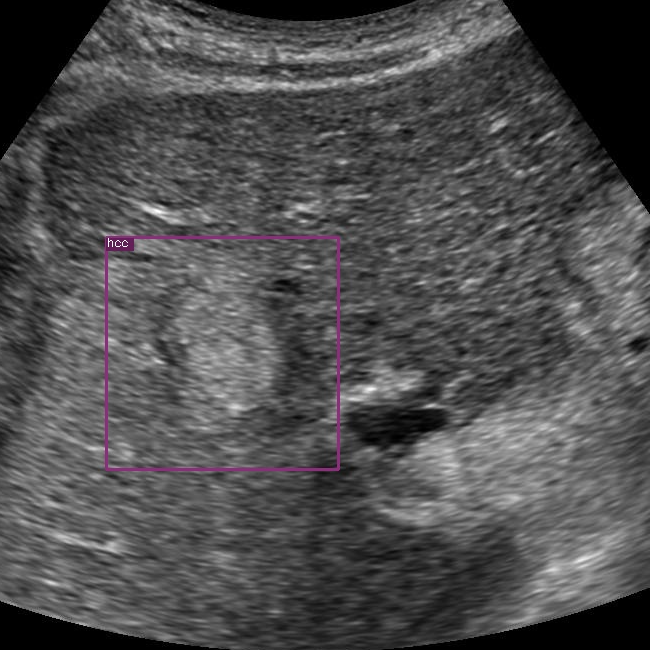
\includegraphics[width=.32\linewidth]{../fig/000814_label.png} \label{fig:hcc_lael}}
        \subfloat[YOLOX]{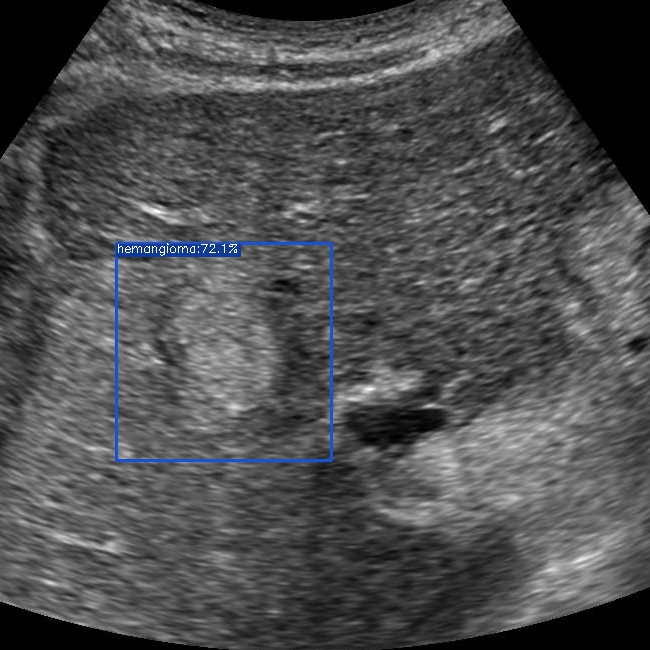
\includegraphics[width=.32\linewidth]{../fig/000814_yolox.png} \label{fig:hcc_yolox}}
        \label{fig:000814}
        \caption{000814.jpgの検出結果}
    \end{figure}

    \begin{thebibliography}{9}
        \bibitem{double_descent} Anonymous authors. \href{https://openreview.net/attachment?id=B1g5sA4twr&name=original_pdf}{DEEP DOUBLE DESCENT: WHERE BIGGER MODELS AND MORE DATA HURT} ICLR 2020, 2020.
        \bibitem{yolox} Zheng Ge, Songtao Liu, Feng Wang, Zeming Li, and Jian Sun. \href{https://arxiv.org/pdf/2107.08430.pdf}{YOLOX: Exceeding YOLO Series in 2021}, 2021.
        \bibitem{simclr} Ting Chen, Simon Kornblith, Mohammad Norouzi, Geoffrey Hinton. \href{https://arxiv.org/pdf/2002.05709.pdf}{A Simple Framework for Contrastive Learning of Visual Representations}, 2020.
        \bibitem{centernet} Xingyi Zhou, Dequan Wang, Philipp Krähenbühl.
        \href{https://arxiv.org/pdf/1904.07850.pdf}{Objects as Points}, 2019.
        \bibitem{simsiam} Xinlei Chen, Kaiming He. \href{https://arxiv.org/pdf/2011.10566.pdf}{Exploring Simple Siamese Representation Learning}, 2020.
    \end{thebibliography}
\end{document}